\chapter{Human-computer interaction}
\label{ch:Human-computer interaction}
Human-computer interaction is a multi-disciplinary research area that includes: user interface design, hardware, software, social aspects and more. Important concepts in this research area are usability and user experience.

With new technology such as novel input devices and increased computational power comes new possibilities. The present work makes use of these new possibilities. Novel user input devices are used for structural modeling, and increased computational power is used for real-time structural analysis. 

\section{Direct manipulation}
Direct manipulation is a human-computer interaction style with continuous representation of objects of interest with rapid, reversible and incremental feedback \cite{Shneiderman1982}. Users can directly manipulate objects on the screen using real-world metaphors, which makes the users more engaged with their task and encouraged to further explorations \cite{Shneiderman:1997:DMC:238218.238281}. This is achieved through reducing the perceptual and cognitive resources required to understand and use the user interface \cite{Sears1990}.

\section{Visualizations}
Scientific visualization is a subfield of computer graphics. The purpose of scientific visualizations is to graphically illustrate scientific data. This is also important for any conceptual structural design software to be successful, how the result is visualized is of great importance. The result should be visualized in a way so that the user quickly can interpret the result and gain insight from it. 

\begin{figure}
  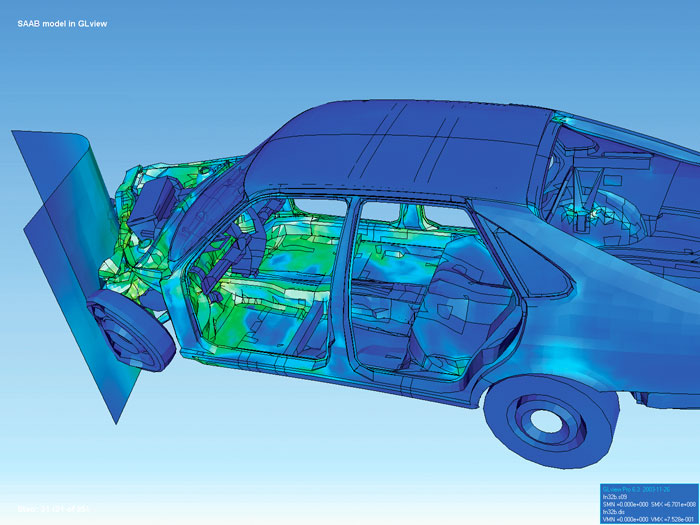
\includegraphics[width=320pt]{graphics/car.jpg}
  \caption{Visualization of how a car deforms in an asymmetrical crash using finite element analysis.}
  \label{fig:Car}
\end{figure}

In Figure \ref{fig:Car} is an example of how the result from a computational analysis often is performed. The original geometry, an undeformed car, is modified with the computed displacement. The geometry, in this case the car, is also colored according to some selected condition. The color can for example represent von Mises tensions, shear forces, bending moment etc. 

Edward Tufte is one of the pioneers in the field of data visualization with his books on information design \cite{tufte1997visual, tufte1990envisioning, tufte2001the}. He has in \cite{tufte2001the} written a few principles of graphical excellence which he stated as follows:

\begin{itemize} 
\item Graphical excellence is the well-designed presentation of interesting data – a matter of substance, of statistics and design.
\item Graphical excellence consists of complex ideas communicated with clarity, precision and efficiency.
\item Graphical excellence in that which gives to the viewer the greatest number of ideas in the shortest time with the least ink in the smallest space.
\end{itemize} 

\section{Technology}
The introduction of different input devices such as the mouse and joystick significantly improved the human-computer interaction of user interfaces that adapted accordingly \cite{Sears1990}. When the touch screen was introduced it had an advantage over all these devices. The user could literally touch objects on the screen to manipulate them, creating a very direct method of inputting information\cite{Sears1990}. This closed the gap between the human and the computer.

There is a wide repertoire of interaction techniques to create direct manipulation user interfaces for three-dimensional (3D) applications using two-dimensional (2D) input devices such as the mouse \cite{Nielson:1987:DMT:319120.319134}. However, since this type of input devices have one degree of freedom less than the 3D user interface there will always exist a need of gestures or similar methods. 

The Leap Motion controller \cite{LeapMotion2013}, is a relatively small and simple input device that is placed in front of the users keyboard, it then tracks the users hands that are in the controllers field of vision. Combined with the software development kit (SDK), the controller creates a computational model of the users hands, which can then be used to interact with software in 3D. This enables very direct manipulations for 3D user interfaces.

Computer games have seen an increase in the amount of novel input devices along with a new style of games to address some limitations of conventional systems \cite{Kosmadoudi2013}, e.g. the Wii remote \cite{Nintendo}, Microsoft’s Kinect for Xbox \cite{Microsoft} and PlayStation Move \cite{Playstationa}. These novel input devices move away from the conventional human-computer interaction to invoke an intuitive interaction that supports the natural human way of working. Games have for long been perceived as fun and engaging, and it has been investigated in many different disciplines if gaming methods can improve the human-computer interaction. In order to create more effective, immersive and engaging learning or training \cite{Kosmadoudi2013}. 

Interest for and development of virtual reality glasses have recently increased, and products such as the Oculus Rift \cite{Oculus} and PlayStation’s Project Morpheus \cite{Playstation}, have recently become widely available. This type of virtual reality glasses has primarily been developed for games but other fields have also shown interest, e.g. in \cite{fogarty2014exploring} a virtual reality is used to help students understand complex structural behavior.
